\documentclass[conference]{IEEEtran}

\usepackage{cite}
\usepackage{amsmath,amssymb,amsfonts}
\usepackage{algorithm}
\usepackage{algpseudocode}
\usepackage{fontspec}
\usepackage{fancyhdr}
\usepackage{graphicx}
\usepackage{booktabs}
\usepackage{array}
\usepackage{textcomp}
\usepackage{xcolor}
\usepackage{url}
\usepackage{lettrine}
\usepackage{float}

\def\BibTeX{{\rm B\kern-.05em{\sc i\kern-.025em b}\kern-.08em
    T\kern-.1667em\lower.7ex\hbox{E}\kern-.125emX}}

\IfFontExistsTF{Times New Roman}
  {\setmainfont{Times New Roman}}
  {\setmainfont{TeX Gyre Termes}}

\renewcommand{\LettrineFontHook}{}
\raggedbottom

\pagestyle{fancy}
\fancyhf{}
\renewcommand{\headrulewidth}{0pt}
\renewcommand{\footrulewidth}{0pt}
\fancyfoot[C]{{\footnotesize Makalah II4021 Kriptografi, Semester II Tahun 2025/2026}}

\makeatletter
\def\section{\@startsection{section}{1}{\z@}{2.2ex plus 1.8ex minus 0.6ex}%
{1.0ex plus 1ex minus 0ex}{\normalfont\normalsize\centering\scshape}}%
\def\subsection{\@startsection{subsection}{2}{\z@}{1.8ex plus 1.5ex minus 0.5ex}%
{0.9ex plus .5ex minus 0ex}{\normalfont\normalsize\itshape}}%
\def\subsubsection{\@startsection{subsubsection}{3}{\parindent}{0ex plus 0.1ex minus 0.1ex}%
{0ex}{\normalfont\normalsize\itshape}}%
\makeatother

\newcommand{\ulineurl}[1]{\url{#1}}

\begin{document}

\title{A Fault-Tolerant Cryptographic Key Recovery\\
Framework Using Reed-Solomon-Decoded\\
Threshold Secret Sharing}

\author{\IEEEauthorblockN{Nayaka Ghana Subrata -- 13523090\textsuperscript{1,2}}
\IEEEauthorblockA{\textit{Department of Informatics Engineering} \\
\textit{School of Electrical Engineering and Informatics} \\
\textit{Institut Teknologi Bandung, Jl. Ganesha 10, Bandung 40132, Indonesia} \\
{\normalfont \textsuperscript{1}\underline{13523090@std.stei.itb.ac.id}, \textsuperscript{2}\underline{nayakaghana39@gmail.com}}}
}

\maketitle
\thispagestyle{empty}
\vspace{0.5em}

\begin{abstract}
\textbf{Cryptographic systems depend on secret keys, yet storing a key in a single location creates a single point of failure. If the key is lost, encrypted data becomes unrecoverable; if the key is copied broadly, the risk of unauthorized disclosure increases. This paper implements and evaluates a fault-tolerant key recovery framework that combines Shamir Secret Sharing with Reed-Solomon-style Berlekamp-Welch decoding. An AES-256 key is first used to protect data with AES-GCM and is then divided into threshold shares over a prime finite field. During recovery, the reconstruction stage can tolerate missing shares and can also correct a limited number of corrupted shares when sufficient redundancy is available. A modular Python prototype is developed to support key generation, authenticated encryption, share creation, robust reconstruction, and experiment automation. Across fifteen experimental scenarios and 375 total trials, all observed outcomes matched the theoretical threshold and decoding bounds. Recovery succeeded in every scenario that satisfied the required redundancy condition and failed in every scenario that violated it. The results show that Reed-Solomon-decoded reconstruction improves availability and fault tolerance without weakening the threshold secrecy property provided by Shamir Secret Sharing.}
\end{abstract}

\begin{IEEEkeywords}
Shamir Secret Sharing, Reed-Solomon Codes, Berlekamp-Welch Decoding, AES Key Recovery, Threshold Cryptography, Robust Secret Sharing
\end{IEEEkeywords}

\section{Introduction}

\lettrine[lines=3,lhang=0.08,loversize=0.15,findent=0.5em,nindent=0em]{T}{he} operational security of symmetric cryptography depends on secret keys. When an encryption key is stored in a single database, device, or password vault, the entire protection mechanism depends on the continued availability and integrity of that one location. The failure modes are immediate: key loss makes ciphertext permanently unreadable, while key compromise allows an attacker to decrypt all protected data. For this reason, practical key management must address both confidentiality and recoverability.

Threshold secret sharing offers a direct way to remove this single point of failure. Shamir's scheme divides a secret into multiple shares such that any threshold number of shares can reconstruct the secret, while any smaller set reveals no information about it \cite{shamir1979}. The construction reduces the access-control problem to polynomial interpolation over a finite field. However, standard reconstruction assumes that the shares presented by participants are correct. In realistic settings this assumption is weak: shares may be unavailable, corrupted by storage faults, or intentionally modified by an adversary.

The close algebraic relationship between Shamir sharing and Reed-Solomon codes makes it natural to strengthen reconstruction with error correction \cite{reedsolomon1960}. Both mechanisms evaluate a low-degree polynomial at distinct field points. As a result, robust recovery can be formulated as recovering the original polynomial from noisy point evaluations, which is precisely the setting addressed by Reed-Solomon decoding algorithms. In particular, the Berlekamp-Welch perspective allows reconstruction to remain correct even when a bounded number of submitted shares are wrong \cite{fedorenko2005}.

This paper studies a practical key recovery prototype rather than a new cryptographic primitive. The protected secret is an AES-256 key \cite{fips197}, used with the AES-GCM authenticated encryption mode \cite{sp80038d}. The contribution lies in implementing a modular end-to-end system and experimentally validating the threshold and error-correction behavior of the resulting recovery process.

The main contributions of this work are as follows:
\begin{enumerate}
\item A modular Python implementation that integrates AES-GCM encryption, Shamir share generation, and Reed-Solomon-style Berlekamp-Welch reconstruction into a single key recovery workflow.
\item An experimental evaluation over fifteen recovery scenarios that cover normal recovery, minimum-threshold recovery, insufficient-share failure, and recovery with corrupted shares.
\item A grounded analysis showing that robust decoding improves availability and fault tolerance without reducing the secrecy threshold of the original sharing scheme.
\end{enumerate}

The remainder of the paper is organized as follows. Section II reviews the necessary theoretical background on AES-GCM, finite-field arithmetic, Shamir sharing, Reed-Solomon codes, and Berlekamp-Welch decoding. Section III presents the proposed recovery framework. Section IV describes the implementation. Section V defines the experiments, while Section VI reports the results and discusses their implications. Section VII analyzes the security model and limitations. Section VIII concludes the paper.

\section{Theoretical Background}

\subsection{AES-GCM}

The Advanced Encryption Standard (AES) is a NIST standard block cipher with 128-bit block size and key sizes of 128, 192, and 256 bits \cite{fips197}. This work uses AES-256 because the goal is not only to split a secret but also to protect a realistic high-value key. Encryption is performed with Galois/Counter Mode (GCM), which provides confidentiality together with integrity through authenticated encryption \cite{sp80038d}. In the prototype, the data owner first encrypts a plaintext under AES-GCM and then protects the resulting AES key with the threshold recovery mechanism.

\subsection{Finite-Field Arithmetic}

Shamir sharing and Reed-Solomon decoding both operate over a finite field. Let $\mathbb{F}_{p}$ be a prime field where all additions, subtractions, multiplications, and inverses are taken modulo a prime $p$. The prototype uses the NIST P-384 prime field, which is larger than the 256-bit AES key space and therefore allows an AES-256 key to be embedded directly as a field element without fragmentation.

Given coefficients $a_{0}, a_{1}, \ldots, a_{d} \in \mathbb{F}_{p}$, a polynomial is written as
\begin{equation}
f(x) = a_{0} + a_{1}x + a_{2}x^{2} + \cdots + a_{d}x^{d}.
\label{eq:polynomial}
\end{equation}
Polynomial evaluation and interpolation are efficient over $\mathbb{F}_{p}$, which makes the field suitable both for share generation and for robust reconstruction.

\subsection{Shamir Secret Sharing}

In a standard $(t,n)$ Shamir scheme, the secret $s$ is stored as the constant term of a random polynomial of degree $t-1$:
\begin{equation}
f(x) = s + a_{1}x + a_{2}x^{2} + \cdots + a_{t-1}x^{t-1},
\label{eq:shamir}
\end{equation}
where $a_{1}, \ldots, a_{t-1}$ are chosen uniformly from $\mathbb{F}_{p}$ \cite{shamir1979}. A share is the pair
\begin{equation}
(x_{i}, y_{i}) = (x_{i}, f(x_{i})).
\label{eq:share}
\end{equation}
Any set of $t$ valid shares uniquely determines $f(x)$, and therefore the secret is recovered by evaluating
\begin{equation}
s = f(0).
\label{eq:secret}
\end{equation}
If fewer than $t$ shares are known, the missing coefficients remain unconstrained, so the secret remains information-theoretically hidden \cite{shamir1979}.

\subsection{Lagrange Reconstruction}

When no share corruption is present, recovery uses interpolation. Given $t$ valid shares $(x_{1},y_{1}), \ldots, (x_{t},y_{t})$, the polynomial can be written in Lagrange form as
\begin{equation}
f(x) = \sum_{i=1}^{t} y_{i}\ell_{i}(x),
\label{eq:lagrange_poly}
\end{equation}
where
\begin{equation}
\ell_{i}(x) = \prod_{\substack{1 \leq j \leq t \\ j \neq i}} \frac{x-x_{j}}{x_{i}-x_{j}}.
\label{eq:lagrange_basis}
\end{equation}
Substituting $x=0$ yields the secret directly:
\begin{equation}
s = f(0) = \sum_{i=1}^{t} y_{i}\ell_{i}(0).
\label{eq:lagrange_secret}
\end{equation}
This formula is sufficient when all submitted shares are valid, but it fails to provide protection against undetected errors in the $y$ values. That limitation motivates the use of Reed-Solomon decoding during reconstruction.

\subsection{Reed-Solomon Codes}

Reed-Solomon codes also encode information by evaluating a low-degree polynomial at multiple field points \cite{reedsolomon1960}. This structural similarity is the key link used in this paper:
\begin{equation}
\text{Shamir sharing} \Longleftrightarrow \text{secure polynomial sharing},
\end{equation}
\begin{equation}
\text{RS decoding} \Longleftrightarrow \text{recovery from noisy shares}.
\end{equation}
For a degree-$(t-1)$ polynomial evaluated at $n$ points, the associated Reed-Solomon code has minimum distance
\begin{equation}
d_{\min} = n - t + 1.
\label{eq:distance}
\end{equation}
This quantity explains the asymmetry between missing and corrupted shares. Missing shares only reduce the number of equations, so recovery requires at least $m \geq t$ available shares. Corrupted shares are harder because the decoder must both identify errors and recover the polynomial, which requires extra redundancy. In coding-theoretic terms, unique decoding can tolerate up to $\lfloor (d_{\min}-1)/2 \rfloor$ symbol errors when all $n$ evaluations are present.

\subsection{Berlekamp-Welch Decoding}

To recover from corrupted shares, this work adopts a Reed-Solomon-style Berlekamp-Welch approach \cite{fedorenko2005}. Suppose a degree-$(t-1)$ polynomial is observed through $m$ shares, of which at most $e$ are corrupted. Correct recovery is possible when
\begin{equation}
m \geq t + 2e.
\label{eq:bound}
\end{equation}

The decoder searches for an error-locator polynomial $E(x)$ of degree $e$ and a combined polynomial $Q(x)$ such that
\begin{equation}
Q(x_{i}) = y_{i}E(x_{i})
\label{eq:bw_constraint}
\end{equation}
for all received shares $(x_{i}, y_{i})$. If a solution exists and $E(x)$ divides $Q(x)$, then the original secret polynomial is recovered as
\begin{equation}
f(x) = \frac{Q(x)}{E(x)}.
\label{eq:quotient}
\end{equation}
The role of $E(x)$ is to vanish at erroneous evaluation points, while $Q(x)$ absorbs the discrepancy between the correct polynomial values and the corrupted observations. In practice the decoder solves a linear system for the unknown coefficients of $Q(x)$ and the non-leading coefficients of $E(x)$, then verifies that the quotient has the expected degree. This verification step is important because it rejects inconsistent share sets instead of silently returning an arbitrary polynomial.

The Reed-Solomon component improves robustness rather than secrecy. It corrects a bounded number of wrong shares, but an adversary who gathers at least $t$ valid shares can still reconstruct the secret by design. This separation between confidentiality and fault tolerance is central to the interpretation of the experimental results.

\section{Proposed Key Recovery Framework}

The proposed framework protects an AES-256 key through threshold sharing while extending the recovery phase with Reed-Solomon-style error correction. The complete workflow has eight stages:
\begin{enumerate}
\item Generate a random AES-256 key.
\item Encrypt the target plaintext with AES-GCM.
\item Convert the AES key to an integer in $\mathbb{F}_{p}$.
\item Split the integer secret into $n$ Shamir shares with threshold $t$.
\item Distribute or store the shares across independent locations.
\item During recovery, collect $m$ available shares.
\item Apply robust reconstruction to tolerate missing or corrupted shares.
\item Use the recovered key to decrypt the ciphertext and verify correctness.
\end{enumerate}

The ordering of these steps matters. The plaintext is encrypted before the key is split so that the recovery procedure handles only a short fixed-size secret rather than an arbitrarily large message. This keeps the secret-sharing layer compact and ensures that the cost of robust reconstruction depends on the key-management problem instead of on the size of the protected data.

Fig.~\ref{fig:workflow} illustrates the end-to-end workflow from AES key generation to robust share-based recovery.

\begin{figure*}[!t]
\centering
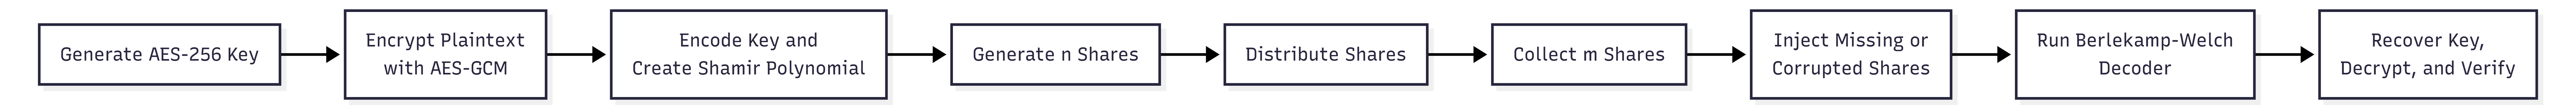
\includegraphics[width=0.96\textwidth,height=2.1in,keepaspectratio,trim=20 20 20 20,clip]{../images/scheme.png}
\caption{End-to-end workflow of the proposed robust AES key recovery framework.}
\label{fig:workflow}
\end{figure*}

Algorithm~\ref{alg:recovery} summarizes the recovery logic. The key observation is that the framework does not replace Shamir's access policy; it refines only the reconstruction stage. If the available shares are all valid, robust recovery reduces to ordinary polynomial interpolation. If a bounded number of shares are corrupted and the redundancy condition in \eqref{eq:bound} holds, the Berlekamp-Welch step recovers the intended polynomial and therefore the original AES key.

\begin{algorithm}[!t]
\caption{Robust AES Key Recovery}
\label{alg:recovery}
\begin{algorithmic}[1]
\Require Threshold $t$, total shares $n$, available shares $\mathcal{S}$, AES-GCM ciphertext package $C$
\Ensure Recovered AES key $K$ or failure
\State Generate a random AES-256 key $K$
\State Encrypt plaintext with AES-GCM under $K$ to obtain $C$
\State Encode $K$ as field element $s \in \mathbb{F}_{p}$
\State Create degree-$(t-1)$ Shamir polynomial $f(x)$ with constant term $s$
\State Distribute $n$ shares $(x_{i}, f(x_{i}))$
\State Collect available shares $\mathcal{S}$ during recovery
\If{$|\mathcal{S}| < t$}
    \State \Return failure
\EndIf
\State Use Berlekamp-Welch decoding on $\mathcal{S}$ to recover $\hat{f}(x)$
\State Extract $\hat{s} = \hat{f}(0)$ and convert it to $\hat{K}$
\State Attempt AES-GCM decryption of $C$ with $\hat{K}$
\If{decryption and authentication succeed}
    \State \Return $\hat{K}$
\Else
    \State \Return failure
\EndIf
\end{algorithmic}
\end{algorithm}

\subsection{Design Assumptions and Parameter Selection}

The framework assumes that the AES key is generated with cryptographically secure randomness and that shares are stored across distinct failure domains. In this setting the threshold $t$ controls the balance between confidentiality and recoverability. A smaller threshold improves availability because fewer shareholders are required during recovery, but it also lowers the number of compromised shares needed for disclosure. A larger threshold has the opposite effect.

The total share count $n$ controls the redundancy budget. When no corruption is expected, the basic reconstruction requirement is only $m \geq t$. When corrupted shares are possible, the choice of $n$ should allow the intended recovery set to satisfy \eqref{eq:bound}. For example, if the design target is to tolerate one corrupted share in a $(3,n)$ system while still recovering from all available shares, then $n$ should be at least $5$. If the target is to tolerate two corrupted shares in a $(5,n)$ system, then at least $9$ shares must participate in reconstruction.

This design targets a specific threat model. It tolerates accidental share loss, partial share compromise below the threshold, and bounded corruption during recovery. It does not claim resistance against an attacker who already possesses at least $t$ valid shares, nor does it protect a workstation that is compromised after the key has been reconstructed.

\section{Implementation}

\subsection{Software Architecture}

The prototype is implemented in Python 3.12 and organized into modular components:
\begin{itemize}
\item \texttt{aes\_utils.py}: AES-256 key generation, AES-GCM encryption and decryption, and conversion between byte strings and field elements.
\item \texttt{field.py}: prime-field arithmetic, polynomial evaluation, and polynomial division helpers.
\item \texttt{shamir.py}: random polynomial generation, share creation, ordinary secret reconstruction, share selection, and share corruption simulation.
\item \texttt{robust\_rs.py}: modular Gaussian elimination, Berlekamp-Welch decoding, and robust secret recovery.
\item \texttt{experiments.py}: automated scenario execution and timing collection.
\end{itemize}

This split keeps cryptographic operations, algebraic utilities, and experiment control separate. The layout also makes it easier to replace the reconstruction method in future work, for example with verifiable or authenticated secret sharing variants.

\subsection{Finite-Field and Serialization Choices}

The implementation uses the NIST P-384 prime field in order to embed a 256-bit AES key directly into one field element. This avoids splitting the key into multiple blocks while still keeping the field size reasonably compact. Shares are serialized using fixed-width field encoding for both the $x$ and $y$ coordinates. As a result, each coordinate occupies 48 bytes and each share occupies 96 bytes in the current prototype. This decision simplifies the implementation and makes storage-overhead calculations deterministic, although a more compact representation for the $x$ coordinate is possible.

\subsection{Recovery Logic}

The decoder accepts the set of available shares and automatically tries the largest feasible error budget first, namely $\lfloor (m-t)/2 \rfloor$, before falling back to smaller budgets. For a fixed error count $e$, the implementation solves the linear system induced by \eqref{eq:bw_constraint}, reconstructs $Q(x)$ and $E(x)$, divides the polynomials, and verifies that the quotient has degree less than $t$. The reconstructed constant term is then converted back into a 32-byte AES key. As a final correctness check, AES-GCM decryption must also succeed, which ensures that an algebraically plausible but incorrect secret is rejected.

\section{Experimental Design}

\subsection{Scenarios}

The evaluation focuses on correctness, decryption success, failure behavior, timing, and storage overhead. Fifteen scenarios were selected to cover both the threshold property and the Reed-Solomon correction bound. Each scenario was executed for 25 independent trials, giving 375 total runs.

Table~\ref{tab:scenarios} lists the evaluated configurations. The ``available'' count $m$ denotes the number of shares presented to the decoder, while $e$ denotes the number of shares intentionally corrupted before recovery. Scenarios marked as failure are expected to fail either because $m < t$ or because the redundancy condition $m \geq t + 2e$ is not satisfied.

\begin{table*}[!t]
\caption{Experimental Scenarios and Observed Outcomes Across 25 Trials Per Scenario}
\label{tab:scenarios}
\centering
\scriptsize
\begin{tabular}{p{2.7in}cccccc}
\toprule
\textbf{Scenario} & \textbf{$t$} & \textbf{$n$} & \textbf{$m$} & \textbf{$e$} & \textbf{Observed Success Rate} & \textbf{Mean Recovery (ms)} \\
\midrule
Normal recovery & 3 & 5 & 5 & 0 & 100\% & 0.1419 \\
Minimum valid recovery & 3 & 5 & 3 & 0 & 100\% & 0.0736 \\
Insufficient shares & 3 & 5 & 2 & 0 & 0\% & 0.0017 \\
One corrupted share, enough redundancy & 3 & 5 & 5 & 1 & 100\% & 0.1781 \\
One corrupted share, not enough redundancy & 3 & 5 & 4 & 1 & 0\% & 0.0402 \\
Larger normal recovery & 4 & 7 & 7 & 0 & 100\% & 0.2937 \\
Larger minimum recovery & 4 & 7 & 4 & 0 & 100\% & 0.1375 \\
Larger insufficient shares & 4 & 7 & 3 & 0 & 0\% & 0.0018 \\
Correct one corrupted share & 4 & 7 & 6 & 1 & 100\% & 0.2397 \\
Correct two corrupted shares & 4 & 8 & 8 & 2 & 100\% & 0.4009 \\
Large threshold normal & 5 & 10 & 10 & 0 & 100\% & 0.6451 \\
Large threshold minimum & 5 & 10 & 5 & 0 & 100\% & 0.1254 \\
Large threshold insufficient & 5 & 10 & 4 & 0 & 0\% & 0.0018 \\
Large threshold, one corrupted & 5 & 10 & 7 & 1 & 100\% & 0.2841 \\
Large threshold, two corrupted & 5 & 10 & 9 & 2 & 100\% & 0.4787 \\
\bottomrule
\end{tabular}
\end{table*}

\subsection{Measurement Procedure}

Each trial follows the same procedure. First, a fresh AES-256 key is generated and used to encrypt a benchmark plaintext with AES-GCM. Second, the key is split into shares under the specified $(t,n)$ configuration. Third, a random subset of $m$ shares is selected. Fourth, the scenario optionally corrupts $e$ of those shares by modifying their $y$ values. Finally, the recovery stage attempts to reconstruct the key and decrypt the ciphertext. Success is recorded only when the recovered key exactly matches the original key and AES-GCM verification succeeds.

Timing is measured separately for share generation and for recovery. Storage overhead is computed as the total serialized share size divided by the original 32-byte AES key size. Because the serialization format is fixed-width, the overhead depends only on the number of generated shares.

\subsection{Evaluation Metrics}

Five metrics are used in the evaluation. First, \textit{recovery success} records whether the robust decoder returns a candidate secret without violating the algebraic constraints. Second, \textit{key correctness} checks whether the recovered 32-byte value matches the original AES key exactly. Third, \textit{decryption success} checks whether AES-GCM accepts the recovered key and reproduces the original plaintext. Fourth, \textit{recovery latency} measures the wall-clock time of the reconstruction stage. Fifth, \textit{storage overhead} measures the total share footprint relative to the 32-byte secret.

These metrics distinguish between algebraic recovery and application-level recovery. In principle a decoder might output a field element even when it is not the original key. By checking both exact key equality and authenticated decryption, the evaluation rejects such cases. This distinction is important because a key-recovery system is useful only when the recovered secret is operationally valid for the protected ciphertext.

\section{Results and Discussion}

\subsection{Functional Verification}

The first result is categorical: every scenario behaved exactly as predicted by theory. Across 375 total trials, all 275 trials in theoretically valid scenarios produced the correct AES key and successfully decrypted the ciphertext, while all 100 trials in theoretically invalid scenarios failed during robust reconstruction. No case produced a false positive decryption.

This outcome directly matches the two central recovery rules:
\begin{itemize}
\item If there are no corrupted shares, recovery succeeds whenever at least $t$ shares are available.
\item If up to $e$ shares are corrupted, recovery succeeds only when $m \geq t + 2e$.
\end{itemize}

The corrupted-share scenarios are especially important because they distinguish the proposed method from ordinary threshold interpolation. For example, the $(t,n,m,e)=(3,5,5,1)$ scenario succeeded in all trials, whereas the $(3,5,4,1)$ scenario failed in all trials because the available redundancy was one share short of the theoretical bound.

\subsection{Failure Behavior}

The invalid scenarios failed for structural rather than incidental reasons. In all runs with $m<t$, the decoder had too few constraints to identify the degree-$(t-1)$ polynomial. In all runs with $m<t+2e$, the system lacked the redundancy needed to both identify the corrupted positions and reconstruct the correct polynomial. The implementation therefore raised decoding failure instead of returning a candidate key. This behavior is desirable because a key-recovery mechanism should fail conservatively when the mathematical recovery conditions are not satisfied.

The absence of false positives is particularly important in the corrupted-share setting. A naive reconstruction procedure that interpolates directly on all submitted points can produce a syntactically valid field element even when one or more shares are wrong. In contrast, the robust decoder in this study couples polynomial consistency checks with AES-GCM verification, so the recovery pipeline accepts only secrets that are algebraically and cryptographically consistent with the original instance.

\subsection{Timing Behavior}

The timing results show two consistent patterns. First, recovery is faster when the number of available shares is close to the minimum threshold, because the decoder solves a smaller linear system. Second, recovery time increases as either the threshold or the correctable error budget grows. This is visible when comparing the mean recovery times in Table~\ref{tab:scenarios}: the smallest successful configuration, minimum valid recovery with $(3,5,3,0)$, required only 0.0736 ms on average, while the largest successful no-error configuration, $(5,10,10,0)$, required 0.6451 ms.

The error-correction overhead is present but modest at the tested scale. For threshold $t=4$, moving from a normal full-share recovery $(4,7,7,0)$ to a two-error correction setting $(4,8,8,2)$ increased mean recovery time from 0.2937 ms to 0.4009 ms. Likewise, for threshold $t=5$, correcting two corrupted shares with nine available shares required 0.4787 ms on average. These values remain well below one millisecond, indicating that the algebraic overhead of robust reconstruction is practical for key-recovery workloads.

The failure cases in Fig.~\ref{fig:timing} also have a useful performance interpretation. Their measured latency is close to zero not because recovery becomes cheaper in a meaningful operational sense, but because the decoder terminates early once the share set is recognized as algebraically insufficient. This means that the additional redundancy required for robust recovery mainly affects the successful path, while invalid configurations are rejected with minimal extra computation.

\begin{figure}[H]
\centering
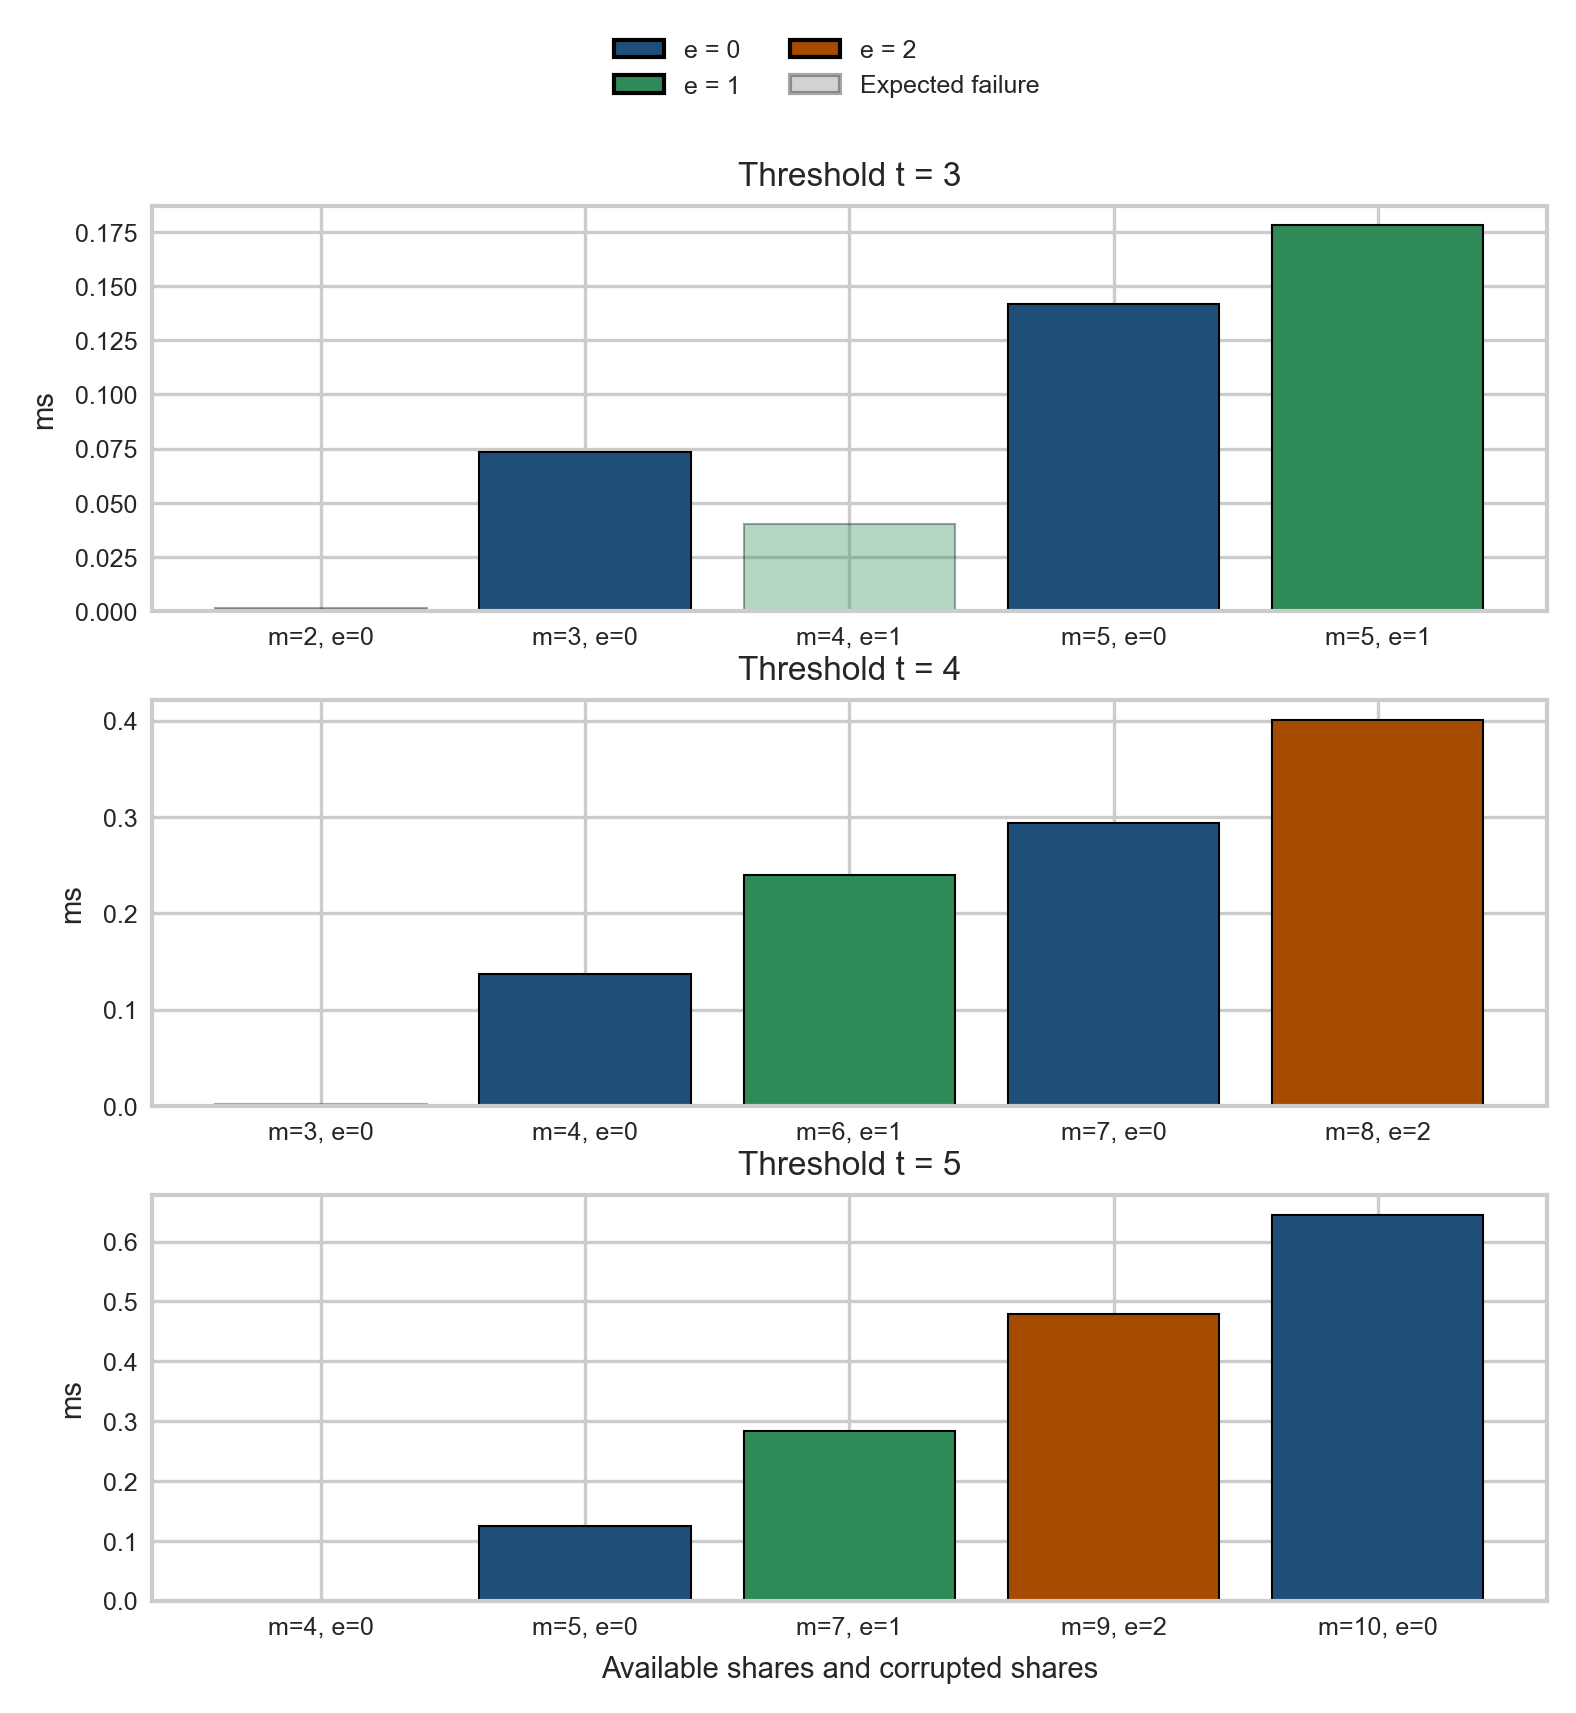
\includegraphics[width=\columnwidth,height=0.88\columnwidth,keepaspectratio]{../images/latency.png}
\caption{Mean recovery latency across threshold settings. Darker bars denote successful configurations, while faded bars denote expected failure cases.}
\label{fig:timing}
\end{figure}

\subsection{Storage Overhead}

Table~\ref{tab:storage} summarizes storage overhead under the fixed-width share format. Because each share occupies 96 bytes, overhead grows linearly with the number of generated shares. This is a predictable trade-off: the prototype gains fault tolerance and distribution flexibility at the cost of storing more total material than the original 32-byte key.

\begin{table}[H]
\caption{Storage Overhead in the Prototype}
\label{tab:storage}
\centering
\begin{tabular}{cccc}
\toprule
\textbf{$n$} & \textbf{Bytes/Share} & \textbf{Total Bytes} & \textbf{Overhead} \\
\midrule
5 & 96 & 480 & 15.0$\times$ \\
7 & 96 & 672 & 21.0$\times$ \\
8 & 96 & 768 & 24.0$\times$ \\
10 & 96 & 960 & 30.0$\times$ \\
\bottomrule
\end{tabular}
\end{table}

Although these ratios appear large compared with the original key size, the absolute storage volume remains small in practical terms. Even the largest configuration stores less than one kilobyte of share data. This is acceptable for archival key protection, password-vault backup, escrow, or multi-party administrative recovery workflows.

\subsection{Interpretation}

The results illustrate the separation between security and robustness. Increasing the threshold strengthens resistance against partial compromise but also reduces the minimum number of missing shares the system can tolerate. Adding Reed-Solomon decoding does not change that threshold policy; instead, it adds resilience against faulty inputs during reconstruction. Shamir sharing determines the access structure, whereas Reed-Solomon decoding determines the level of reconstruction fault tolerance.

Another noteworthy observation is that failure is clean. In every invalid scenario, the decoder rejected the share set rather than silently producing a usable but wrong AES key. This behavior is important because a fault-tolerant recovery system should fail closed when the algebraic constraints are unsatisfied.

The storage and timing measurements also indicate where the practical costs of the approach lie. The storage overhead is dominated by the field representation of the shares rather than by the AES key itself. The computational overhead is concentrated in the decoder, especially as the threshold and error budget grow. For the current parameter range, neither cost is prohibitive, but both would become more significant in deployments with very large thresholds or frequent reconstruction operations. This suggests that the design is best suited to backup, escrow, archival recovery, and administrative key-management settings rather than to high-frequency online use.

\section{Security Analysis}

The confidentiality of the framework is inherited from Shamir Secret Sharing. Any adversary who obtains fewer than $t$ valid shares learns no information about the protected AES key beyond what is already possible without the shares \cite{shamir1979}. This is an information-theoretic guarantee of the sharing scheme and does not depend on computational hardness assumptions.

The Reed-Solomon component serves a different role. It improves availability and robustness by correcting a bounded number of corrupted shares during recovery, but it does not reduce the threshold needed to determine the secret polynomial. Therefore, it is incorrect to claim that Reed-Solomon decoding strengthens secrecy. Its benefit is operational: it allows the honest recovery process to survive a limited amount of data corruption.

\subsection{Adversarial Capabilities}

The analysis assumes that an adversary may observe, steal, delete, or modify a subset of stored shares. The adversary may also submit malformed shares during reconstruction in an attempt to induce decoder failure or to force recovery of an incorrect secret. However, the adversary is not assumed to break AES-GCM directly, invert finite-field operations, or compromise the randomness used to generate the Shamir polynomial. These assumptions match the intended application of the framework as a key-management and recovery mechanism rather than as a replacement for the underlying symmetric cipher.

The framework addresses four practical risks:
\begin{enumerate}
\item \textit{Single point of failure:} no single location stores the entire AES key.
\item \textit{Key loss due to partial unavailability:} recovery remains possible as long as the threshold or decoding bound is satisfied.
\item \textit{Partial share compromise:} fewer than $t$ valid shares do not reveal the secret.
\item \textit{Limited share corruption:} bounded tampering can be corrected when enough redundancy is available.
\end{enumerate}

At the same time, several limitations remain:
\begin{enumerate}
\item If an attacker acquires at least $t$ valid shares, the key is recoverable by design.
\item If the reconstruction endpoint is compromised, the attacker may steal the recovered AES key after successful recovery.
\item The current prototype assumes reliable share authenticity is not provided externally. A malicious actor can still force denial of service by injecting too many invalid shares.
\item Share storage remains meaningful only if the shares are actually separated across different administrative or physical domains.
\end{enumerate}

\subsection{Mitigations and Extensions}

Several extensions would strengthen the framework in deployment. Verifiable secret sharing can help participants detect incorrect shares before interpolation, while authenticated or signed share containers can make the corruption source easier to identify \cite{cheraghchi2019}. Operationally, share placement policies should ensure that independent shares are not stored in a single cloud account, server cluster, or administrative domain. Reconstruction should also occur only on a trusted endpoint, because the threshold mechanism protects the stored key but not a machine that is already compromised at the moment of recovery.

\section{Conclusion}

This paper presented a practical key recovery framework that combines Shamir Secret Sharing with Reed-Solomon-style Berlekamp-Welch decoding. The implementation protects an AES-256 key by distributing it into threshold shares and reconstructing it robustly in the presence of missing or corrupted inputs. A modular Python prototype was developed and evaluated on fifteen scenarios covering nominal recovery, threshold-limited failure, and corrupted-share recovery.

The experimental results matched the theoretical bounds exactly across 375 trials. Recovery succeeded in every valid scenario and failed in every invalid scenario, while mean recovery times remained below one millisecond for all tested configurations. These findings show that robust reconstruction can improve the availability of threshold key management without weakening its confidentiality guarantees.

Future work can extend the prototype with share authentication, verifiable secret sharing, compact serialization, and larger-scale performance measurements. The present results already show that coding-theoretic decoding can be integrated into threshold key recovery without altering the underlying secrecy threshold.

\section*{Acknowledgment}

Praise and gratitude are offered to Allah SWT, whose blessings and grace enabled the completion of this paper. Special thanks are extended to Dr. Ir. Rinaldi Munir, M.T., for his guidance and teaching throughout the author's studies in the sixth semester, including II4021 Cryptography, which supported the completion of this work. The author also expresses sincere gratitude to his parents for their constant support and encouragement.


\bibliographystyle{IEEEtran}
\bibliography{references}
\section*{Repository}

The implementation code, experimental scripts, and document source for this paper are publicly available at the following GitHub repository:

\begin{center}
\underline{\url{https://github.com/Nayekah/reed-solomon-secret-sharing}}
\end{center}

\section*{Statement}

I hereby declare that this paper is my own work, is not a translation or reproduction of another person's paper, and is not plagiarized.

\begin{flushright}
Bandung, May 18\textsuperscript{th} 2026

\vspace{0.7em}
\includegraphics[width=1.1in]{../images/signature.png}

\vspace{0.4em}
Nayaka Ghana Subrata\\
13523090
\end{flushright}


\end{document}
